\graphicspath{{chapters/images/01/}}
\chapter{\emph{Escherichia Coli} general informations}

\section{\emph{E. coli} genomics}
\emph{Escherichia Coli} is a Gram-negative, facultative anaerobic, rodshaped, coliform bacterium, it pertains to the phylum of proteobacteria and to the family of Enterobacteriaceae. It can be grown easily and inexpensively. Its genome has a length between $4.5$-$4.7Mb$, including about $4000$-$5000$ genes, and about seven ribosomal RNA operons. Only the $38\%$ of the genes of K-12 (one of the most studied bacterial strains of \emph{E. coli}) were experimentally identified, overall $40$-$50\%$ of the genes are to date without a known function.
The original \emph{E. coli} strain K-12 was obtained from a stool sample of a diphtheria patient in Palo Alto, California in 1922.

    \subsection{\emph{E. coli} long-term evolution experiment}
    The \emph{E. coli} long-term evolution experiment led by Richard Lenski is one of the longest evolutionary experiments ever made.
    Starting from the 24th of Frbruary 1988 $12$ population of E. coli have been cultivated in parallel.
    After each day a portion of the population was introduced in a new flask, where it proliferated.
    Every $500$ generations a sample from each flask is saved, so to track the evolutionary changes made.
    Today the $66000th$ generation have been reached.
    Long-term adaptation to a fixed environment can be characterized by a rich and dynamic set of population genetic processes, instead of the evolutionary desert expected near a fitness optima.
    In particular some bacteria developed the capacity to aerobically grow on citrate.

    \subsection{\emph{E. coli} strains}
    \emph{E. coli} could be found as commensal strains, pathogenic strains, or environmental strains. The pathogenic strains could pertain to these categories (which are not exclusive):

    \begin{multicols}{2}
        \begin{itemize}
            \item enteropathogenic (EPEC),
            \item enteroinvasive (EIEC),
            \item enterotoxigenic (ETEC),
            \item diffusely adherent (DAEC),
            \item adherent invasive (AIEC),
            \item shiga-toxin producing (STEC),
            \item enteroaggregative(EAEC),
            \item extraintestinal pathogenic (ExPEC).
        \end{itemize}
    \end{multicols}

    Resistances to antibiotics adds another layer of complexity in the categorization categorization of \emph{E. coli}.
    Most of the genes are on plasmids, circular, additional to chromosome, and can be moved easily horizontally. Plasmids between different strains can be moved in enterobacteriacae, this doesn't happen normally in other families.
    Some \emph{E. coli} strains are even capable of causing cancer in humans: for example, colibactin-positive \emph{E. coli} can cause colon and rectal cancer, by creating mutations which are responsible of the of the cancer onset.

    \subsection{Stc-EAEC outbreak}
    In 2011 in Germany there was an outbreak of Stx-EAEC,
    An efficient counter-measure was found by sequencing the genome of those bacteria.

    \subsection{Shigella}
    Shigella is a strain of \emph{E. coli} capable of producing the shiga toxin.
    It has been difficult to categorize for taxonomists.
    Several antigens can be used by taxonomists to categorize \emph{E. coli} strains.
    In particular the O ($171$), H ($56$), K ($80$) antigens, respectively related to the somatic, the flagella and the capsule are widely used.

    \subsection{PanPhlAn - strain detection and characterization}
    Pangenome-based Phylogenomic Analysis (PanPhlAn) is a strain-level metagenomic profiling tool for identifying the gene composition and in-vivo transcriptional activity of individual strains in metagenomic samples.
    PanPhlAn’s ability for strain-tracking and functional analysis of unknown pathogens makes it an efficient tool for culture-free infectious outbreak epidemiology and microbial population studies.
    This tool was for example used to study the strain responsible of an outbreak in Germany in 2011 and found a strain of shiga-toxigenic Escherichia coli (STEC).
    This method, due to its greater efficiency and accuracy has been used since instead of low-throughput, traditional pipelines.

\section{Genomes of \emph{E. coli}}

    \subsection{Core and accessory genome}
    In the genome of \emph{E. coli} strains, it is possible to distinguish between:

    \begin{multicols}{2}
        \begin{itemize}
            \item Core genome: the set of all genes shared by all members of a bacterial species, it includes 1000 up to 3000 genes.
            \item Accessory or dispensable genome: the set of genes present in some but not all genomes within the same bacterial species.
                It is found on a single strain or in a subset of strains.
        \end{itemize}
    \end{multicols}

    \subsection{Pangenome}
    The pangenome is the union of the core genome and the accessory genome.
    It is the set of all the set of all the genes that can be found in the species strains.
    The pangenome can be characterized regarding its size with respect to the number of genomes:

    \begin{multicols}{2}
        \begin{itemize}
            \item Closed: the pangenome size tends to a maximum as number of genomes increases.
            \item Open: the pangenome size keeps increasing as you add new genomes.
        \end{itemize}
    \end{multicols}

    Typically sequencing more organisms of the same species tends to lower the amount of genes in the core genome and increase the number of those in the pangenome, \ref{corepangenome}.
    Due to technical errors, the core genome should tend to a size of $0$, but a more reasonable plateau can be predicted with a more accurate mathematical formulation.

    \begin{figure}[h]
    \centering
    \includegraphics[width=0.6\textwidth]{genesSharedDifferentGenomes}
    \caption{It can be seen that $51\%$ of the genes are strain specific, and the other are shared between 2 to 20 strains of \emph{E. coli}}
    \label{corepangenome}
    \end{figure}

    Each \emph{E. Coli} genome contains a balance genes of the core genome and of the pan genome, for a total amount of $4700$ genes \ref{balancepancore}).
    Core genomes' genes are responsible of some basic cellular functionalities and utilities to survive the environment, while instead elements of the pangenome are quite usually specific to a single strain, like for example antibiotic resistance, and they are often not functionally well characterized.

    \begin{figure}[h]
    \centering
    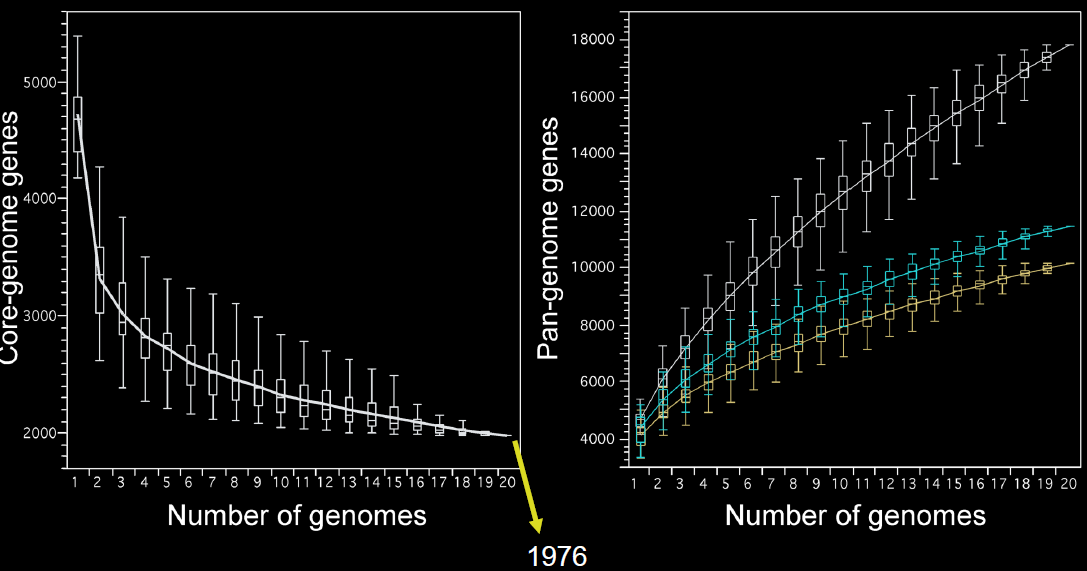
\includegraphics[width=8cm]{corePanGenEcoli}
    \caption{Balance between genes of the core- and of the pan-genome}
    \label{balancepancore}
    \end{figure}
